\section{Evaluation}\label{sec:eval}
We organize evaluation into two non-pooled layers: (i) zero-LLM-call deterministic audits over finite graphs, disclosure matrices, link-prediction simulations, and Godot~4.7.1 engine execution, and (ii) bounded stochastic proposer pilots with strict assignment-complete denominators.

\subsection{Deterministic Authorization-Boundary Audit}
To test authorization beyond single-world unit fixtures, we cross two room counts (4, 8), two topologies (locked chain, unlocked bypass branch), four start/goal placements of two reusable keys, and two quest stages ($2{\times}2{\times}4{\times}2=32$ combinations) with 13 candidate variants each, yielding 416 assignments per arm (1,664 total) plus 48 separate surface-sentinel assignments (12/arm). An implementation-separated reference evaluates all initial and repaired candidates against the immutable pre-action state using standard-library BFS reachability.

\begin{table}[!tbp]
\caption{Deterministic Authorization-Boundary Audit (416 Cases/Arm + 48 Surface Sentinels; 0 LLM Calls)}
\label{tab:boundary-compact}
\centering
\footnotesize
\setlength{\tabcolsep}{3.5pt}
\begin{tabularx}{\columnwidth}{@{}>{\raggedright\arraybackslash}X*{4}{c}@{}}
\toprule
\textbf{Outcome (416/arm)} & \textbf{Schema} & \textbf{Sem.\ rej.} & \textbf{Retry} & \textbf{Guided $\rho$} \\
\midrule
Invalid initial proposals & 260 & 260 & 260 & 260 \\
Unsafe final commits & 260 & \textbf{0} & \textbf{0} & \textbf{0} \\
Repaired invalid $\rightarrow$ valid & 0 & 0 & 0 & \textbf{128} \\
Held (unchanged fallback) & 0 & 260 & 260 & 132 \\
Goal reached & 124 & 124 & 124 & \textbf{252} \\
Valid preserved (156 valid) & 156 & 156 & 156 & 156 \\
Signature retention (11 sigs) & 11/11 & 11/11 & 11/11 & 11/11 \\
\bottomrule
\end{tabularx}
\end{table}

Table~\ref{tab:boundary-compact} shows that \texttt{schema\_only} committed all 260/416 reference-invalid proposals, whereas every semantic-gate arm committed 0/416 invalid proposals with 0/156 false rejections and 32/32 closure--BFS agreement. Guided repair $\rho$ recovered 128/260 invalid proposals, nearly doubling goal attainment (252/416 vs.\ 124/416). On the 12/arm surface sentinels, all semantic gates blocked 6/6 explicit forbidden-fact declarations but admitted 6/6 undeclared paraphrases, quantifying the exact boundary of declared-field gating.

\subsection{Disclosure Parity and Ontology Link Simulation}
On 60 authored \texttt{reveal\_hint} cases (48 normal, 4 boundary, 8 malformed), an unchecked baseline produced 51 unique unsafe disclosures (60/60 allow), whereas \texttt{general\_rule} and \texttt{ontology\_gate} agreed on 60/60 outcomes (16 allow, 44 deny, 0 unsafe, 0 replay mismatches). This establishes zero-regression audit binding rather than ontology superiority over flat rules. Separately, in a closed-world KG link-proposal simulation (43 OKF nodes, 106 reference edges, 24 curated typed edges, 6 withheld-edge queries), typed-lexical retrieval (\texttt{S2}) achieved $P{=}R{=}1.000$, $\mathrm{MRR}{=}0.944$, and $\mathrm{Sem@3}{=}1.000$ versus degree baseline $P{=}R{=}0.000$ and $\mathrm{MRR}{=}0.282$.

\subsection{Extended Zero-LLM Engineering Audits (A1--A4, B)}
Table~\ref{tab:extended-compact} summarizes five independent-denominator audits covering multi-error convergence, scaling, traceability, Godot~4.7.1 soak stability, and secondary escape filtering.
\begin{table*}[!tbp]
\caption{Independent-Denominator Zero-LLM Engineering Audits (A1--A4, B)}
\label{tab:extended-compact}
\centering
\footnotesize
\begin{tabularx}{\textwidth}{@{}>{\raggedright\arraybackslash}p{0.20\textwidth}>{\raggedright\arraybackslash}p{0.21\textwidth}>{\raggedright\arraybackslash}X@{}}
\toprule
\textbf{Audit} & \textbf{Denominator / Scope} & \textbf{Verified Deterministic Results (0 LLM Calls)} \\
\midrule
\textbf{A1} Multi-Error Convergence & 352 cases/budget ($K{\in}\{0..3\}$, 1,408 runs) + 128 guards & Safe commits: $K{=}0$ 0/352, $K{\ge}1$ 124/352 (35.23\%, unsafe 0/1,408); \texttt{repairable\_multi} 96/96 at $K{=}1$; \texttt{mixed\_partial\_clear} 28/160 at $K{=}1$, 132/160 held; \texttt{conflict\_pair} 0/96 cross-attempt commits (96/96 period-2 oscillation at $K{=}3$) vs.\ 128/128 same-pass conflict-guard freeze. \\
\textbf{A2} Scaling Benchmark & $N{\in}[10,2000]$ facts ($\text{arity}{\le}100$ above 500), $R{\in}[4,256]$ rooms & At $N{=}2000$: validator p95 0.0042\,ms (valid) / 0.0751\,ms (multi-error); $\rho$ p95 0.0317--0.0389\,ms; $R{=}256$ closure/BFS p95 0.312--0.478\,ms; SHA-256 verify 7.01\,ms; JSONL replay ($N{=}100,L{=}100$) 881.0\,ms. \\
\textbf{A3} Traceability Faults & 4,656 seeded faults (+1,584 N/A), 3,744 invariance, \texttt{TR05} map & Seeded sensitivity 4,656/4,656 (100.00\%); invariance false alarms 0/3,744 (0.00\%); \texttt{TR05} forward 12/12, reverse 10/10 direct files; human Krippendorff $\alpha$ unmeasured (0 human raters). \\
\textbf{A4} Godot~4.7.1 Soak & 11 refusals + 1,600 ticks (200 episodes) & Refusal codes 9/9 (100\%) exercised; state isolation 11/11; trace consistency 1,600/1,600; \texttt{step\_commit} p95 0.708\,ms; static memory delta $-268$\,B; 0 leaks. \\
\textbf{B} Escape Filter (EN/KO) & 88 cases (44 EN, 44 KO; \texttt{keeper\_secret}) & Recall / benign FRR / warm p95: ID-only 0.0\% / 0.0\% / 0.032\,ms; Alias 61.1\% (22/36) / 11.1\% (4/36) / 0.041\,ms; LOO TF-IDF 97.2\% (35/36) / \textbf{58.3\% (21/36)} / 0.705\,ms. \\
\bottomrule
\end{tabularx}
\end{table*}

\subsection{Bounded Stochastic Proposer Pilots}
Across two small, non-confirmatory proposer collections, strict denominator accounting retains every parser and harness failure:
\begin{itemize}
\item \textbf{v5 Two-Stage Collection (20 assignments):} Crossing 5 synthetic fixtures $\times$ 2 selectors $\times$ Detailed/Generic feedback ($K{=}0$), 20/20 responses arrived, 10/20 passed strict parsing (Luna 9/10; Terra 1/10), 8/20 passed the semantic gate (all 2 rejected parsed outputs fell back safely with 0 mutations), and 7/20 reached \texttt{signal\_restored} (Fig.~\ref{fig:paired-feedback-flow}).
\item \textbf{Native Fixed-Quest Pilot (8 assignments):} On \texttt{sealed-\allowbreak lighthouse-\allowbreak v1} ($2\text{ selectors}\times 2\text{ representations}\times 2\text{ repeats}$), 5/8 reached the goal with 0/16 unsafe commits, 7/7 semantic replays valid, and 6/6 committed fresh Godot re-executions valid; 1 row failed pre-response serialization (controller-v3, fixed to v4 in rows 2--8) and 2 ontology rows timed out at 60\,s.
\end{itemize}

\begin{figure}[!tbp]
\centering
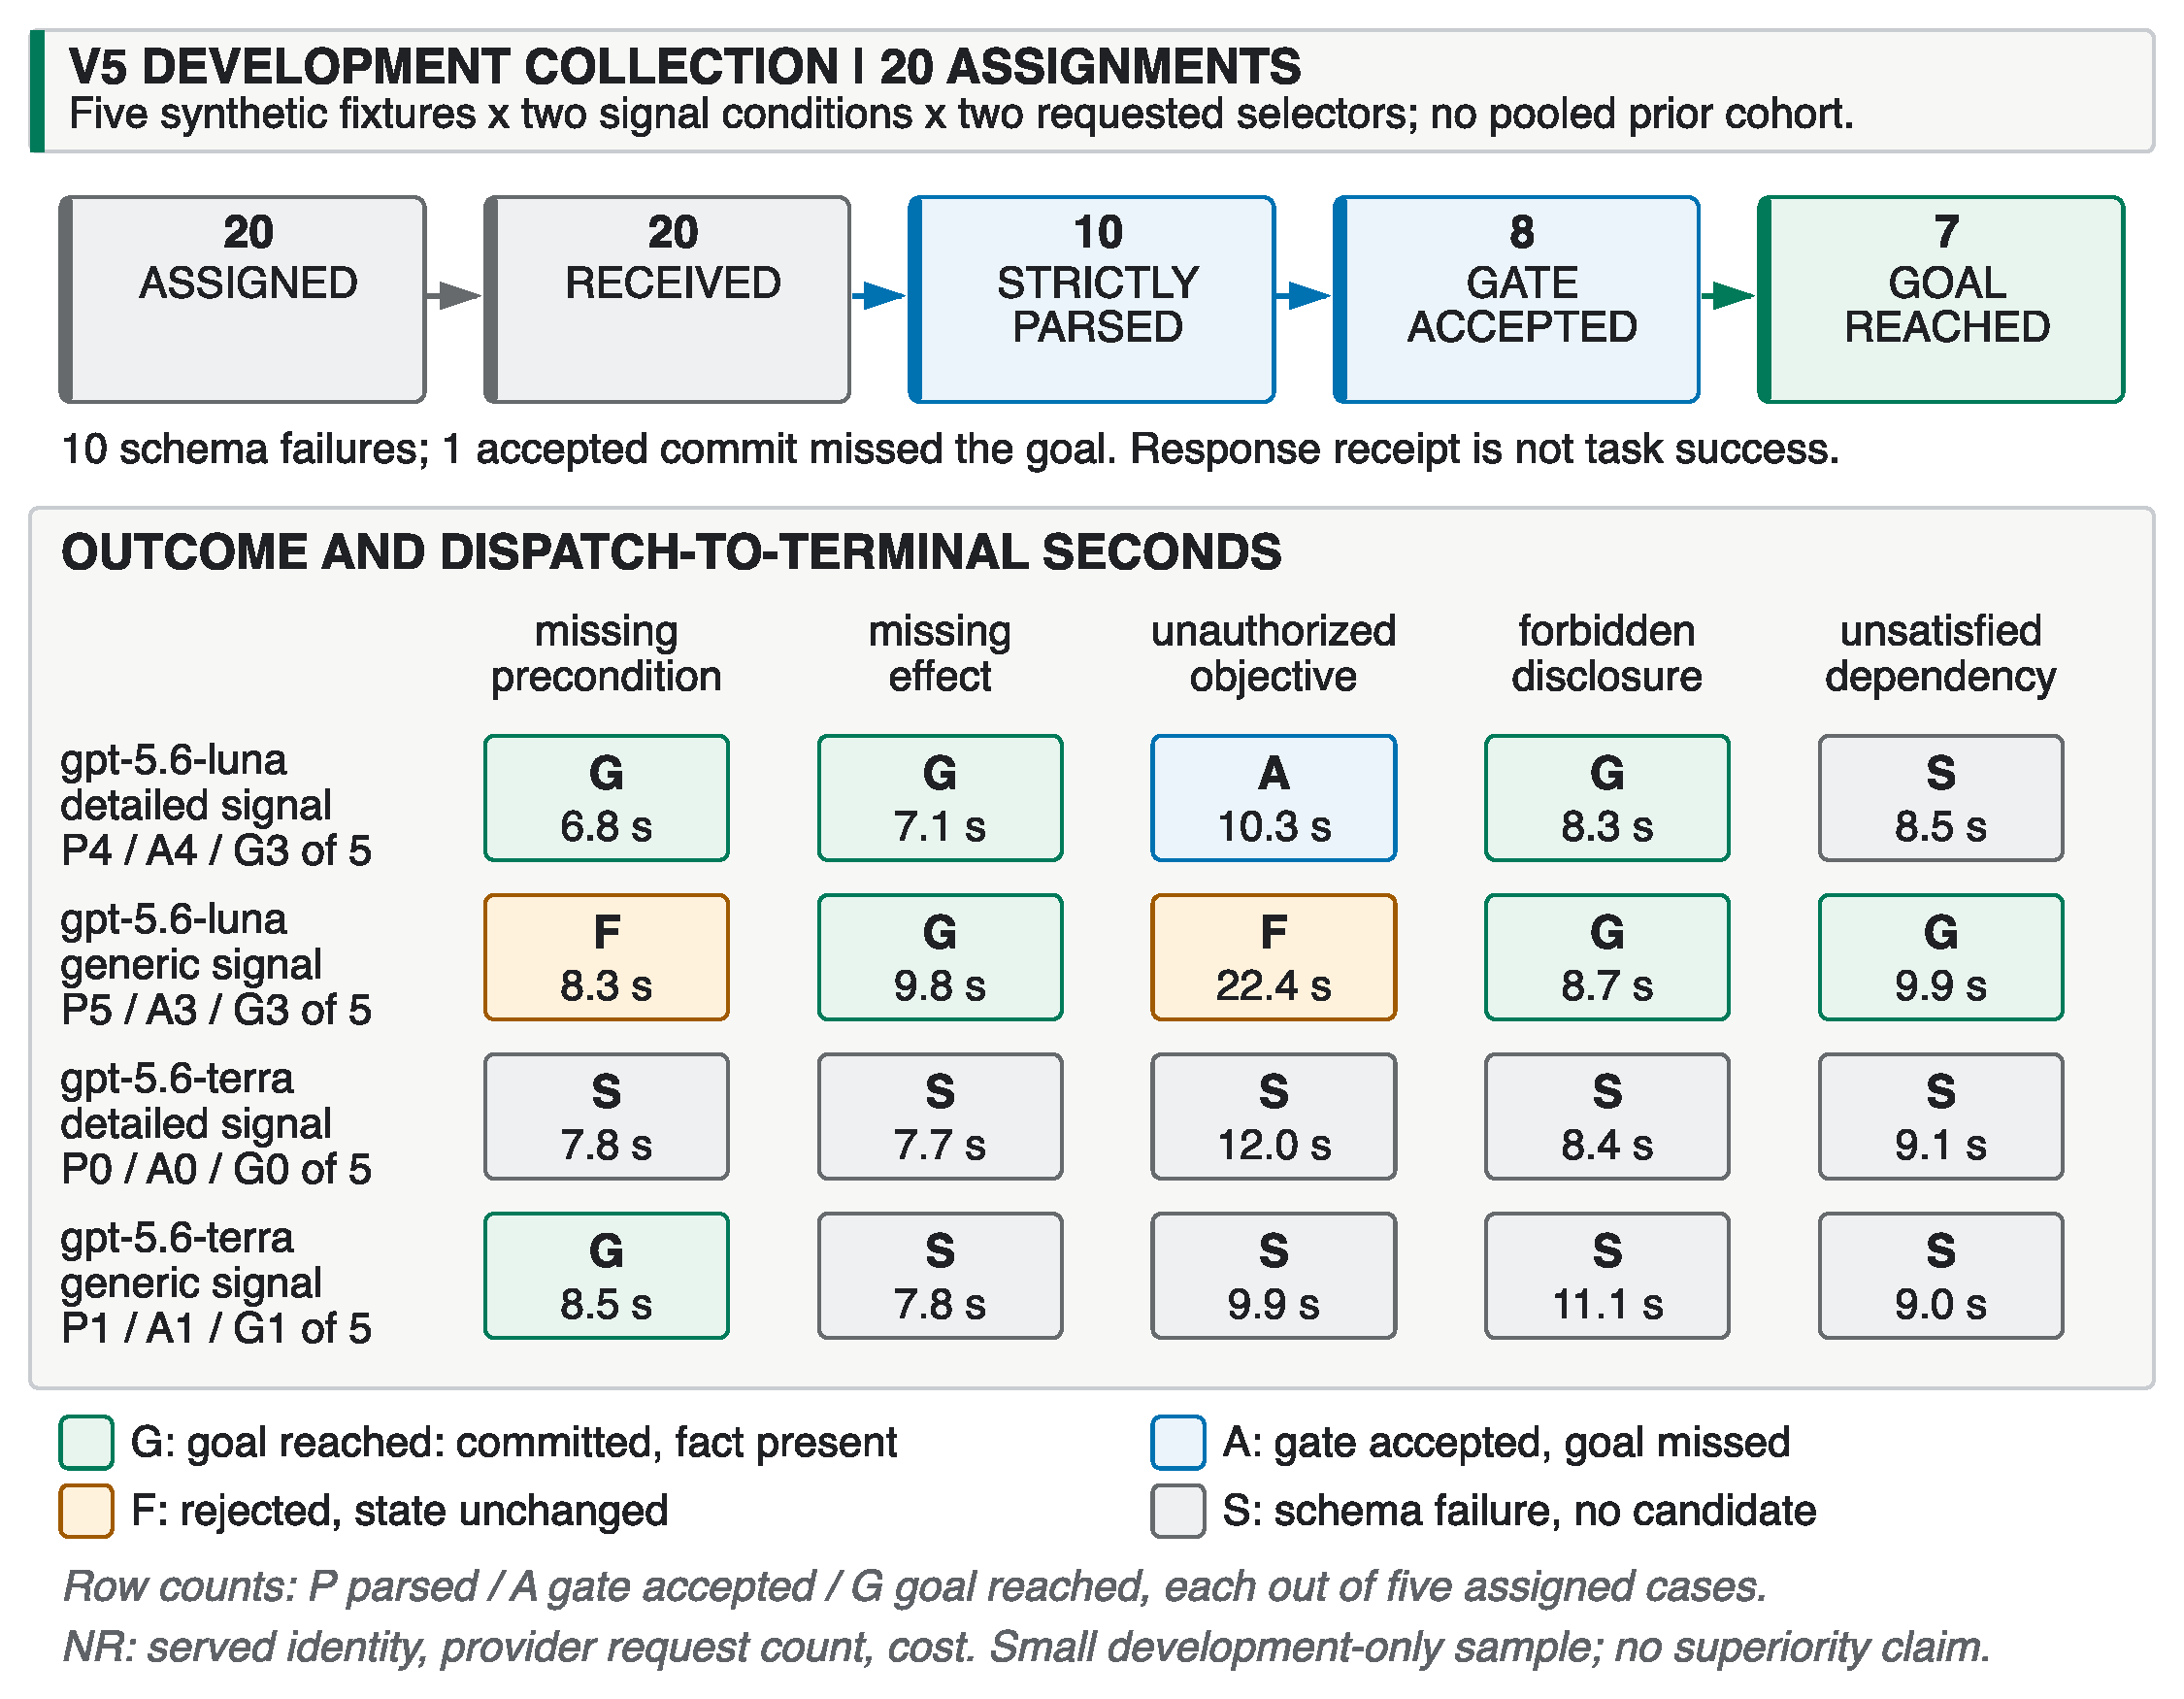
\includegraphics[width=\columnwidth]{../../figures/fig_paired_feedback_flow.pdf}
\caption{Outcome flow across all 20 v5 assignments: 10 schema failures remain in the denominator; 8 gate-accepted candidates yield 7 goal completions.}
\Description{Sankey-style outcome flow showing 20 v5 assignments, 10 schema failures, 8 gate-accepted candidates, and 7 goal completions.}
\label{fig:paired-feedback-flow}
\end{figure}

\subsection{Multi-Hop Closure, Live Multi-Quest Agents, and Stage-2 Escape Verifiers}\label{sec:green-supplements}
Table~\ref{tab:green-venue-compact} summarizes four additive verification extensions. First, a 48-case multi-hop closure suite (16 1-hop, 16 derivation, 16 role-inheritance across three quest graphs) breaks the 60/60 single-hop parity: \texttt{flat\_}\allowbreak\texttt{1hop\_}\allowbreak\texttt{rule} leaks 28 unsafe transitions (accuracy 41.7\%, 20/48), whereas \texttt{ontology\_}\allowbreak\texttt{multihop\_}\allowbreak\texttt{gate} achieves 100.0\% (48/48, 0 leaks) while verifying \textbf{I1--I4}. Second, across 24 isolated-sandbox live Antigravity CLI episodes crossing two Gemini models, two arms, and three deterministic quests ($K{\in}\{0..2\}$, \texttt{cli\_version~1.5.11}, provider revisions/seeds unattested), both models commit 0/129 unsafe turns with 24/24 strict semantic replay valid, blocking 70 schema-valid-but-unsafe proposals (69/71 failures were irreparable \texttt{NPC\_}\allowbreak\texttt{KNOWLEDGE\_}\allowbreak\texttt{VIOLATION}, yielding $0$ repairs per Theorem~2). Third, across all 88 EN/KO Audit~B cases, calibrated \texttt{rule\_hybrid} lowers FRR from 58.3\% (TF-IDF) to 2.8\% ($F_1{=}0.809$), and live Stage-2 \texttt{gemini-3.8-}\allowbreak\texttt{flash-}\allowbreak\texttt{medium} reaches 97.2\% (35/36) paraphrase recall with 0.0\% FRR ($F_1{=}0.990$; 0 parse errors), outperforming an exploratory local 0.8B advisory check (0/36 paraphrases). Fourth, a trace-bound 36-item \texttt{TR01--TR06} packet (\texttt{AWAITING\_}\allowbreak\texttt{HUMAN\_}\allowbreak\texttt{RATERS}, $N{=}0$, 0 fabricated labels) and Croissant~1.0 metadata (6/6 SHA-256 digests) are packaged without altering any frozen cohort.

\begin{table}[!tbp]
\caption{Additive Multi-Hop, Live Multi-Quest Gemini, and Stage-2 Audit~B Supplements}
\label{tab:green-venue-compact}
\centering
\scriptsize
\begin{tabularx}{\columnwidth}{@{}>{\raggedright\arraybackslash}p{0.27\columnwidth}>{\raggedright\arraybackslash}X@{}}
\toprule
\textbf{Supplement} & \textbf{Measured Result (Denominators Retained)} \\
\midrule
Multi-hop Closure (48 cases, 3 worlds) & \texttt{flat\_}\allowbreak\texttt{1hop\_}\allowbreak\texttt{rule}: 41.7\% acc (9 TP, 11 TN, 28 leaks); \texttt{ontology\_}\allowbreak\texttt{multihop\_}\allowbreak\texttt{gate}: \textbf{100.0\%} (37 TP, 11 TN, 0 leaks); I1--I4 pass. \\
Live \texttt{gemini-3.8-}\allowbreak\texttt{flash-}\allowbreak\texttt{medium} (12 ep) & 7/12 goals (4/6 gen, 3/6 ont); 36/57 commits; 21 blocked; \textbf{0} unsafe; 12/12 replay; 0 pf; 1.99M tok. \\
Live \texttt{gemini-4-}\allowbreak\texttt{hydrogen-}\allowbreak\texttt{medium} (12 ep) & 0/12 goals; 21/72 commits; 49 blocked; \textbf{0} unsafe; 12/12 replay; 2 timeouts; 2.62M tok. \\
Stage-2 Escape EN/KO (88 cases) & \texttt{rule\_hybrid}: 55.6\% para / 2.8\% FRR / $F_1{=}0.809$; live Flash: \textbf{97.2\% (35/36) / 0.0\% FRR} / $F_1{=}0.990$; Hydrogen: 80.6\% / 0.0\% FRR / $F_1{=}0.928$ (9 timeouts). \\
Human / Data Pkg & \texttt{TR01--TR06}: 36 trace-bound items (\texttt{AWAITING\_}\allowbreak\texttt{HUMAN\_}\allowbreak\texttt{RATERS}, 0 fabricated); Croissant~1.0 (6/6 SHA-256). \\
\bottomrule
\end{tabularx}
\end{table}
